% ============================================================
% Cheat sheet, argomento: il pattern Singleton (dispensa, capitolo 15)
% ============================================================
\argomento{Singleton}{Dispensa: capitolo 15. Pattern creazionale della GoF}[Pattern Singleton]

\scheda{Carta d'identità}{
  \pintento{Garantire che una classe abbia \textbf{una e una sola istanza}, e dare a tutti un \textbf{punto di
    accesso globale} a quell'istanza.}
  \ptesto{«un solo», «unico», «una e una sola istanza», «condiviso da tutta l'applicazione», «accessibile da
    ovunque»; gli esempi tipici: la \textbf{connessione al database}, la \textbf{configurazione}, il registro dei
    \textbf{log}, la coda di stampa.}
  \pcodice{costruttore \textbf{\code{private}}; un campo \code{private static} del \textbf{tipo della classe stessa};
    un metodo \code{public static getInstance()} che crea l'oggetto solo se il campo è \code{null} e poi restituisce
    sempre quello; spesso \code{clone()} ridefinito per lanciare un'eccezione. Chi lo usa scrive
    \code{Classe.getInstance()}, mai \code{new}.}
  \pdiagramma{una classe sola, con un attributo \underline{sottolineato} del suo stesso tipo, il costruttore con il
    \code{-} e un'operazione \underline{sottolineata} che restituisce la classe.}
  \pvarianti{istanza creata subito, quando la classe viene caricata (\code{private static final Singleton ISTANZA =
    new Singleton();}): niente inizializzazione pigra, ma sicura con i thread; \code{getInstance} con
    \code{synchronized}; un numero \textbf{fisso} di istanze (al massimo 3, in un array: \vv{singleton-varianti});
    un'\code{enum} con un solo valore \oltre.}
  \pconfondere{una classe con soli metodi \code{static} (come \code{Math}): non c'è un oggetto, non si può
    personalizzare la creazione né passarlo come parametro. E la Dependency Injection (\vv{di-struttura}): lì
    l'oggetto viene \textbf{passato} a chi lo usa, qui chi lo usa \textbf{va a prenderlo}.}
}

\begin{struttura}{singleton-struttura}{La struttura}
\begin{tikzpicture}
  \umlclass[4.4cm]{s}{(0,0)}{Singleton}{\underline{- instance: Singleton}}{- Singleton()\\\underline{+ getInstance(): Singleton}}
  \node[notauml, anchor=west, text width=4.3cm] (n) at (2.8,0) {if (instance == null)\\\hspace*{1em}instance = new Singleton();\\return instance;};
  \draw[tratt] (s.east) -- (n.west);
\end{tikzpicture}
\tcblower
\textbf{Un solo partecipante}: la classe stessa. Il campo statico appartiene alla classe e sopravvive mentre gli
oggetti nascono e muoiono; il costruttore privato lo può chiamare solo \code{getInstance}, che lo chiama una volta
sola (\textit{lazy initialization}). Se un'altra classe prova \code{new Singleton()}, la ferma il compilatore:
\code{Singleton() has private access}.
\end{struttura}

\begin{programma}{singleton-esempio}{L'esempio del corso: un nome che non cambia}
\begin{lstlisting}[style=javacs, name=Esecutore.java]
public class Esecutore {
    public static void main(String[] args) {
        SingletonClass sc1 =
                SingletonClass.getInstance("uno");
        SingletonClass sc2 =
                SingletonClass.getInstance("due");
        System.out.println(sc1.getNome()
                + " --- " + sc2.getNome());
        System.out.println("stesso oggetto? "
                + (sc1 == sc2));
    }
}

class SingletonClass {
    private static SingletonClass instance = null;
    private final String nome;

    private SingletonClass(String nome) {
        this.nome = nome;
    }
    public static SingletonClass getInstance(
            String nome) {
        if (instance == null)
            instance = new SingletonClass(nome);
        return instance;
    }
    public String getNome() { return nome; }
}
\end{lstlisting}
\tcblower
\begin{tikzpicture}
  \umlclass[5.6cm]{s}{(0,0)}{SingletonClass}{\underline{- instance: SingletonClass = null}\\- nome: String \{readOnly\}}{- SingletonClass(nome: String)\\\underline{+ getInstance(nome: String): SingletonClass}\\+ getNome(): String}
  \umlclass[3.4cm]{e}{(0,2.4)}{Esecutore}{}{\underline{+ main(args: String [*])}}
  \draw[dep] (e.south) -- node[stereo, right]{«call»} (s.north);
\end{tikzpicture}

\medskip
\begin{lstlisting}[style=shellcs, name=Terminale]
$ javac Esecutore.java
$ java Esecutore
uno --- uno
stesso oggetto? true
\end{lstlisting}
\regola{La seconda chiamata trova \code{instance} già impostato: non chiama il costruttore e il parametro
\code{"due"} viene \textbf{ignorato}. Per questo un \code{getInstance} con parametri è ingannevole: meglio
configurare l'oggetto una volta, all'avvio. (Nel codice del corso \code{nome} è un campo \code{static}; qui è un
campo dell'oggetto, che è la scelta più comune.)}
\end{programma}

\begin{caso}{singleton-varianti}{Le varianti nel codice}
\begin{lstlisting}[style=javacs]
// creato subito, quando la classe viene caricata
class Configurazione {
    private static final Configurazione ISTANZA =
            new Configurazione();
    private Configurazione() { }
    public static Configurazione getInstance() {
        return ISTANZA;
    }
}
// pigro ma sicuro con i thread
class Registro {
    private static Registro istanza;
    private Registro() { }
    public static synchronized Registro
            getInstance() {
        if (istanza == null)
            istanza = new Registro();
        return istanza;
    }
}
// al massimo tre istanze, assegnate a turno
class Stampante {
    private static final Stampante[] istanze =
            new Stampante[3];
    private static int prossima = 0;
    private Stampante() { }
    public static Stampante getStampante() {
        int i = prossima;
        prossima = (prossima + 1) % 3;
        if (istanze[i] == null)
            istanze[i] = new Stampante();
        return istanze[i];
    }
}
\end{lstlisting}
\tcblower
\begin{tikzpicture}
  \umlclass[6.2cm]{c}{(0,0)}{Configurazione}{\underline{- ISTANZA: Configurazione \{readOnly\}}}{- Configurazione()\\\underline{+ getInstance(): Configurazione}}
  \umlclass[5.4cm]{s}{(0,-2.6)}{Stampante}{\underline{- istanze: Stampante [3]}\\\underline{- prossima: int = 0}}{- Stampante()\\\underline{+ getStampante(): Stampante}}
\end{tikzpicture}
\regola{Il diagramma non cambia: costruttore privato, campo e metodo statici. Il campo creato subito è
\code{final}, quindi \code{\{readOnly\}}. Con un numero fisso di istanze il campo è un array: la molteplicità
\code{[3]}.}
\end{caso}
